\documentclass [a4paper,12pt]{book}
\usepackage[italian]{babel}
\usepackage[utf8]{inputenc}
\usepackage[T1]{fontenc}
\usepackage{lmodern}
\usepackage{graphicx}
\usepackage{minted}
\usepackage{tikz}
\usetikzlibrary{shapes,shadows,arrows}
\usepackage{fancyhdr}
\usepackage{epigraph}
\setlength{\epigraphwidth}{33em}
\usepackage{float}
\restylefloat{table}
\usepackage{url}
\usepackage[bookmarks,pdftex,
pdfauthor={Francesco Soncina},
pdftitle={IEEE 802.21: Media Independent Handover},
pdfsubject={IEEE 802.21},
pdfkeywords={IEEE, 802.21, ODTONE, MIHF},
pdfproducer={Latex with hyperref},
pdfcreator={pdflatex}]{hyperref}
\usepackage{booktabs}
\pagestyle{empty}
\newcommand{\cmd}[1]{\\\texttt{#1}\\}
\newcommand{\cmduser}[1]{\\\texttt{\$ #1}\\}
\newcommand{\cmdroot}[1]{\\\texttt{\# #1}\\}
\linespread{1,3}

\title{IEEE 802.21: Media Independent Handover}
\author{Francesco Soncina}
\date{18 Marzo 2014}

\begin{document}
\begin{titlepage}
\thispagestyle{empty}
\begin{center}
\fontsize{16}{0}{\textsc{Alma Mater Studiorum$\cdot$Università di Bologna}}
\rule[0.1cm]{13.3cm}{0.1mm}
\rule[0.5cm]{13.3cm}{0.6mm}
{\small{\bf SCUOLA DI SCIENZE\\
Corso di Laurea in Informatica }}
\end{center}
\vspace{15mm}
\begin{center}
{\LARGE{\bf IEEE 802.21:}}\\
\vspace{3mm}
{\LARGE{\bf Media Independent Handover}}\\
\vspace{19mm} {\large{\bf Tesi di Laurea in Reti di Calcolatori}}
\end{center}
\vspace{40mm}
\par
\noindent
\begin{minipage}[t]{0.47\textwidth}
{\large{\bf Relatore:\\
Chiar.mo Prof.\\
Vittorio Ghini}}
\end{minipage}
\hfill
\begin{minipage}[t]{0.47\textwidth}\raggedleft
{\large{\bf Presentata da:\\
Francesco Soncina}}
\end{minipage}
\vspace{20mm}
\begin{center}
{\large{\bf Sessione III\\%inserire il numero della sessione in cui ci si laurea
2012/2013 }}%inserire l'anno accademico a cui si è iscritti
\end{center}
\end{titlepage}
\frontmatter
%\begin{center}
\thispagestyle{empty}
\vspace{5em}
\LARGE{\textbf{IEEE 802.21:\\ Media Independent Handover}}\\
\vspace{1em}
\Large{Francesco Soncina}\\
\vspace{1em}
\Large {18/3/2014}\\
\end{center}
\maketitle
\pagestyle{fancy}
\epigraph{{\em "I'm personally convinced that computer science has a lot in common with physics. Both are about how the world works at a rather fundamental level. The difference, of course, is that while in physics you're supposed to figure out how the world is made up, in computer science you create the world. Within the confines of the computer, you're the creator. You get to ultimately control everything that happens. If you're good enough, you can be God. On a small scale."}}{Just for Fun\\Linus Torvalds, David Diamond} 


\begin{center}
\LARGE{\textbf{Abstract}}
\end{center}
\vspace{3em}
In questo lavoro, dopo un'introduzione sul panorama contemporaneo, si è analizzato lo standard IEEE 802.21, illustrandone i motivi che hanno portato al suo sviluppo, la {\em timeline} del processo di standardizzazione, gli obbiettivi del {\em working group}, l'architettura del sistema specificato e le sue funzionalità, con particolare riguardo all'utilità in applicazioni reali, al fine di darne un giudizio completo sulla sua effettiva efficacia. Dopo aver citato qualche esempio di possibile applicazione dello standard e descritto lo stato attuale dell'arte, si è studiata una sua implementazione {\em cross-platform} chiamata ODTONE, descrivendone i vari componenti e le loro funzionalità, ma anche sottolineando le attuali mancanze per arrivare ad una implementazione completa sotto tutti i punti di vista. Successivamente si è studiata ed implementata un'applicazione, {\em MIH-proxy}, che potesse sfruttare in modo costruttivo i servizi specificati dallo standard per creare un proxy che potesse scegliere su quale interfaccia instradare i pacchetti a seconda dello stato attuale di tutti i collegamenti, realizzato in versione unidirezionale e bidirezionale. In particolare questa applicazione è in grado di restare in ascolto di cambiamenti di stato delle interfacce di rete, e.g. quando viene stabilita una connessione oppure cade, e, di conseguenza, stabilire di volta in volta quali collegamenti utilizzare per inviare dati. Nella versione bidirezionale è anche possibile far comunicare tra loro applicazioni che normalmente utilizzerebbero il protocollo di trasporto TCP attraverso un ulteriore componente, {\em phoxy}, che si preoccupa di convertire, in modo trasparente, un flusso TCP in datagrammi UDP eventualmente cifrati. Sarà quindi possibile creare un collegamento criptato ad alta affidabilità tra le applicazioni che possa sfruttare tutte le interfacce disponibili, sia per inviare, sia per ricevere.
\tableofcontents
\pagestyle{empty}
\listoffigures
\listoftables
\mainmatter
\pagestyle{fancy}
\chapter{Introduzione}
In questo capitolo verranno esposte le motivazioni e gli obbiettivi di questo lavoro, a partire dalla situazione odierna per descriverne i problemi che hanno portato allo sviluppo dello standard IEEE 802.21.

\section{La situazione odierna}
Il mondo di oggi è in continua evoluzione, ogni giorno abbiamo nuovi dispositivi con hardware sempre migliore non solo sotto un punto di vista qualitativo, bensì anche quantitativo, nel senso che i nuovi {\em devices} hanno sempre più elettronica a bordo per poter sfruttare le nuove tecnologie, in particolare riguardo alla connettività, diventata negli ultimi anni un aspetto fondamentale della vita di tutti i giorni. Il fatto che ormai la maggioranza dei nuovi dispositivi sia dotata di più interfacce di rete spiana la strada a molte opportunità, ma, allo stesso tempo, pone anche degli ostacoli lungo il cammino.
Chiunque possieda uno smartphone recente può connettersi alla rete in più modi, come Wi-Fi, GSM, UMTS, HSDPA, LTE, etc. Se, per esempio, si è attualmente connessi tramite una connessione wireless ed usciamo dalla zona di copertura dell'{\em Access Point}, il {\em device} si collegherà automaticamente attraverso un'altra tecnologia, attivando le ricetrasmittenti adatte oppure se usciamo dalla zona di copertura della nostra attuale connessione GSM, il dispositivo si connetterà autonomamente ad un'altra torretta. L'atto di cambiare l'{\em access point} oppure addirittura la tecnologia utilizzata per ristabilire la connessione è detto {\em handover} e può essere più tipi. La figura \ref{fig:handovers} riassume graficamente quanto detto, mostrando i movimenti di un apparato mobile dotato di connettività Wi-Fi, WiMaX e 3G che, uscendo di volta in volta dal raggio di azione dell'{\em Access Point} a cui è attualmente connesso, adotta le azioni di {\em handover} necessarie per ripristinare la connettività, ristabilendo la connessione sull'interfaccia migliore tenendo conto delle prestazioni del {\em link} ed il consumo energetico associato.

\begin{figure}[h!]
\centering
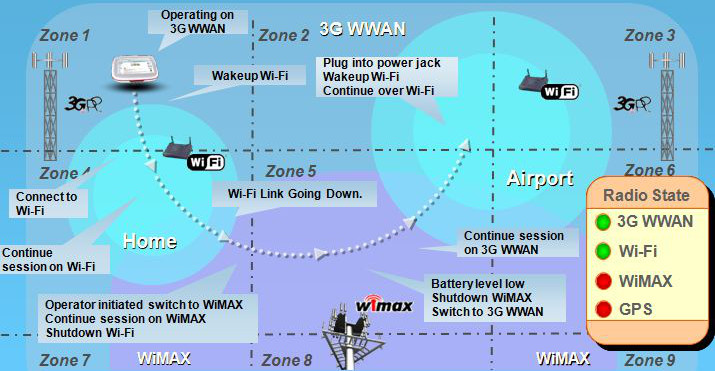
\includegraphics[scale=0.55]{handovers.jpg}
\caption{Handovers}
\label{fig:handovers}
\end{figure}

\section{Tipi di handovers}

I due esempi sopra citati descrivono rispettivamente uno scenario di {\em handover} verticale ed orizzontale, a seconda della tecnologia utilizzata prima e dopo il passaggio. Oltre a questo classificazione, è possibile descrivere altri due tipi di {\em handover}, a seconda che le connessioni aperte al momento del passaggio vengano o meno preservate nel passaggio.

\subsection{Horizontal handover}
Nel caso del telefonino che cambia la propria BTS\footnote{Base Transceiver Station}, quando esce dal raggio di azione della prima, si parla di un {\em handover} orizzontale, i.e. la tecnologia adoperata a livello {\em data link} non cambia. Stesso tipologia di {\em handover} se, muovendoci, ci si collega man mano agli {\em access points} Wi-Fi con miglior ricezione e ciò può anche essere effettuato utilizzando due interfacce 802.11 contemporaneamente in modo da avere potenzialmente entrambe le connessioni attive al momento del passaggio.

\subsection{Vertical handover}
Se è necessario, invece, cambiare il livello {\em data link} durante il passaggio, allora si tratta di un {\em handover} verticale. Sono i più utili da un punto di vista applicativo poiché permettono di sfruttare le diverse caratteristiche intrinseche di ogni particolare tecnologia, ovvero si potrebbe essere interessati ad utilizzare una connessione Wi-Fi qualora disponibile e passare su HSDPA solo quando si esce dalla zona di copertura dell'attuale {\em access point}, in modo da poter mantenere attiva la connessione, anche cambiando il mezzo trasmissivo e, di conseguenza, il livello {\em data link}.

\subsection{Hard handover}
Si tratta di un {\em handover} dove le connessioni attive prima del passaggio vengono chiuse, incaricando il dispositivo stesso di ripristinarle da zero successivamente, quando avrà stabilito con successo un nuovo collegamento. Viene anche definito come {\em break-before-make}.

\subsection{Soft handover}
In questo caso le connessioni aperte vengono mantenute anche dopo il passaggio, in modo da preservare lo stato della rete e consentire un passaggio trasparente ed indolore all'utente. Questo è realizzato stabilendo una connessione verso il nuovo {\em access point} preventivamente, in modo che, prima che il collegamento salti, si abbia già un altro canale pronto all'uso. Viene anche definito come {\em make-before-break}.

\section{Problematiche}
I problemi principali da gestire sono:
\begin{enumerate}
\item come e quando debbano effettuarsi le decisioni di {\em handover}.
\item come debba avvenire effettivamente il passaggio tra {\em access points} della stessa rete, al fine di mantenere lo stato della sessione.
\item come debba avvenire effettivamente il passaggio tra {\em access points} di reti diverse, al fine di mantenere lo stato della sessione.
\end{enumerate}
Lo standard IEEE 802.21, preso in esame in questo lavoro, mira a risolvere il primo problema, fornendo dei servizi {\em media-independent} per prendere le dovute decisioni di {\em handover} in un modo standardizzato ed indipendente dalla tecnologia utilizzata al momento, ma non stabilisce come effettivamente debba avvenire il passaggio.
Per il secondo problema è necessario stabilire opportune specifiche di come debba effettivamente avvenire l'{\em handover} tra {\em access points} della stessa rete, ad esempio come lo standard IEEE 802.11r-2008\cite{ieee80211r} per il passaggio da un {\em access point} Wi-Fi all'altro.
Per il terzo problema è possibile adottare soluzioni come il {\em Mobile IP}\cite{mobileip} dell'IETF\footnote{Internet Engineering Task Force}, il quale permette il {\em routing} dei pacchetti indipendentemente dalla posizione fisica del {\em device} associandogli un indirizzo IP permanente.
\chapter{Lo standard IEEE 802.21}

In questo capitolo sarà esposto lo standard IEEE 802.21\cite{ieee80221}, illustrandone le componenti e le loro funzionalità, al fine di avere un quadro completo e poter comprendere il suo reale obbiettivo, ovvero creare un meccanismo standardizzato per poter prendere più facilmente decisioni di {\em handover}, in modo che sia {\em media-independent}, ovvero indipendente dal mezzo trasmissivo utilizzato.

\section{Storia}
Con il continuo diffondersi di nuove tecnologie e dispositivi dotati di più interfacce di rete, è diventato necessario dover formalizzare alcune funzionalità per facilitare un passaggio indolore da una rete all'altra.
Come possiamo notare dalla figura \ref{fig:timeline}, il {\em working group} cominciò effettivamente i lavori nel marzo 2004 e la prima versione ufficiale dello standard fu pubblicata nel gennaio 2009. Gli eventi principali sono stati i seguenti:
\begin{itemize}
\item marzo 2003: creazione IEEE 802.21 ECSG\footnote{Executive Committee Study Group}
\item marzo 2004: creazione IEEE 802.21 WG\footnote{Working Group}
\item settembre 2004: analisi dei requisiti
\item ottobre 2004: raccolta delle proposte
\item maggio 2005: formulazione di una proposta unica
\item luglio 2005: inizio discussione della proposta
\item luglio 2007: IEEE 802 Sponsor Ballot\cite{balloting}
\item gennaio 2009: pubblicazione dello standard
\end{itemize}

\begin{figure}[h!]
\centering
\hspace*{-1em}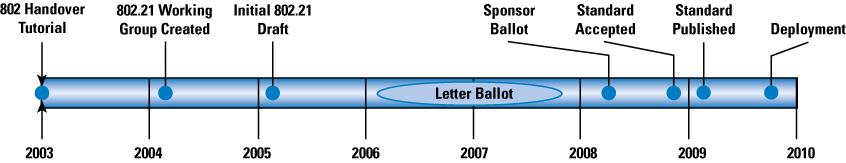
\includegraphics[scale=0.5]{ieee_timeline.jpg}
\caption{IEEE 802.21 Timeline}
\label{fig:timeline}
\end{figure}

\section{Finalità}
Lo standard IEEE 802.21 si pone l'obbiettivo di aiutare i nodi mobili a prepararsi ad eventuali azioni di {\em handover} da un {\em access point} all'altro, ma non specifica come debba avvenire la migrazione. Come sintetizzato dalla figura \ref{fig:rapporto}, esso si pone da intermediario tra gli standards coinvolti in azioni di {\em handover}: sono infatti definite tutte le funzionalità per acquisire informazioni sullo stato delle varie interfacce, ma non è specificato come e quando debba effettivamente avvenire l'eventuale passaggio, il quale ha bisogno di apposite specifiche. L'applicazione utente che usufruisce dei servizi offerti da questo standard è in grado di conoscere lo stato delle connessioni disponibili attraverso la ricezione di eventi dal proprio MIHF\footnote{Media Independent Handover Function}, quali {\em link\_up} e {\em link\_down}, e può, ad esempio, richiedere esplicitamente informazioni aggiuntive su una interfaccia inviando delle specifiche richieste ad un particolare SAP\footnote{Service Access Point}, come l'RSSI\footnote{Received Signal Strength Indication} di una propria interfaccia 802.11 attualmente connessa. Lo standard IEEE 802.21 da solo non basta per gestire interamente i meccanismi di {\em handover}, poiché, ad esempio, per riuscire ad effettuare una migrazione {\em seamless} delle connessioni attualmente attive, mantenendo quindi lo stato dei flussi aperti prima e dopo l'{\em handover}, sarebbe necessaria anche una migrazione dell'indirizzo di terzo livello attraverso, ad esempio, Mobile IP\cite{mobileip}, altrimenti, dopo aver instaurato con successo la nuova connessione, il {\em peer} remoto non potrebbe sapere il nuovo indirizzo del nodo a cui era connesso precedentemente.

\begin{figure}[h!]
\centering
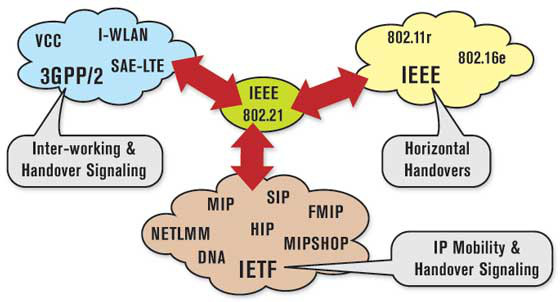
\includegraphics[scale=0.6]{ieee80221_cloud.jpg}
\caption{Rapporto con gli altri standards}
\label{fig:rapporto}
\end{figure}

\section{Architettura}
Lo standard IEEE 802.21 definisce più entità, rappresentate graficamente in figura \ref{fig:80221arch}, ognuna con il proprio specifico compito, al fine di fornire tutti i servizi necessari a prendere decisioni di {\em handover} in modo {\em media-independent}, ovvero in modo indipendente dalla tecnologia utilizzata in quel preciso momento:
\begin{itemize}
\item MIHF: implementa il core delle funzionalità offerte dallo standard.
\item MIH-SAP: fornisce una astrazione {\em media-independent} per tutti i tipi di interfacce.
\item MIH-LINK-SAP: fornisce una astrazione {\em media-specific} per una singola tecnologia.
\item MIH-NET-SAP: permette la gestione di MIHF remoti.
\item MIH-User: è l'entità che si sottoscrive ad un MIHF per usufruire dei servizi offerti.
\end{itemize}

\begin{figure}[h!]
\centering
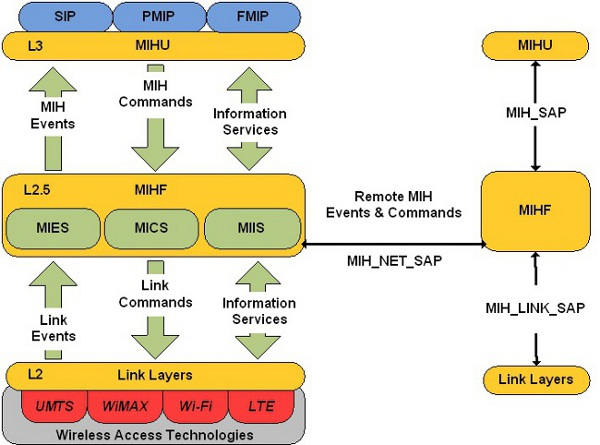
\includegraphics[scale=0.9]{ieee80221.jpg}
\caption{Architettura IEEE 802.21}
\label{fig:80221arch}
\end{figure}
\subsection{MIHF}
Questo componente è il più importante: i nodi mobili devono sottoscriversi ad un MIHF, il quale invierà loro una conferma con informazioni sui collegamenti disponibili, come i rispettivi indirizzi di livello due ed il tipo di tecnologia, ed un elenco di eventi e comandi supportati. Ogni MIHF fornisce un insieme di servizi astratti ai livelli superiori indipendentemente dalle tecnologie adottate dalle singole interfacce gestite.
L'implementazione della Media Independent Handover Function è formata da tre sottocomponenti:

\begin{itemize}
\item MIES (Media Independent Event Services): ha il compito di propagare gli eventi a tutte le parti interessate, come eventuali cambiamenti dello stato a livello {\em data link} agli strati superiori dello stack di rete del sistema locale o di sistemi remoti. Per un elenco completo di tutti gli eventi specificati nello standard IEEE 802.21 ed i loro significati si faccia riferimento alla tabella \ref{mihevents}. Gli eventi possono essere generati dall'MIHF stesso oppure dai livelli sottostanti. Il flusso dei dati generati da questo componente ha quindi un verso prettamente {\em bottom-up}.

\begin{table}[h]
\begin{tabular}{p{0.35\textwidth}|p{0.65\textwidth}}
\toprule
\textbf{Nome} & \textbf{Descrizione} \\
\midrule
Link\_Up & è generato quando una specifica interfaccia diventa attiva, i.e. viene stabilita una connessione di secondo livello\\
\hline
Link\_Down & è generato quando cade una connessione di secondo livello di una specifica interfaccia, e.g. disconnessione da una rete {\em wireless}\\
\hline
Link\_Detected & è generato quando è disponibile una nuova rete di cui usufruire, ad esempio la scoperta di una nuova rete {\em wireless} durante una scansione\\
\hline
Link\_Going\_Down & può essere generato da un SAP per informare le parti interessate che le prestazioni di un dato {\em link} stanno man mano degradando, secondo vari criteri, e.g. pacchetti persi, larghezza di banda, latenza, etc.\\
\hline
Link\_Handover\_Imminent & è utilizzato per comunicare alle entità interessate che sta per essere eseguita una procedura di {\em handover} \\
\hline
Link\_Handover\_Complete & è utilizzato per segnalare alle entità interessate che la procedura di {\em handover} è stata completata con successo\\
\bottomrule
\end{tabular}
\caption{Lista degli eventi specificati nello standard}
\label{mihevents}
\end{table}

\item MICS (Media Independent Command Services): è incaricato di propagare i comandi ricevuti dagli strati più alti dello stack di rete verso il basso per aiutare il nodo mobile ad eseguire più facilmente procedure di {\em handover}, ad esempio una richiesta esplicita di riconfigurazione per un'interfaccia, per comunicare ad un MIHF remoto di procedere con l'esecuzione di un {\em handover} oppure una richiesta di informazioni più dettagliate sullo stato di un collegamento specifico, e.g. richiedere il valore RSSI di un'interfaccia wireless. Per una lista completa di tutti i comandi previsti dallo standard IEEE 802.21 si faccia riferimento alla tabella \ref{mihcommands}. I comandi possono essere originati sia dall'MIH-User, sia dall'MIHF stesso. La destinazione dei comandi può essere per i livelli inferiori dello stack locale oppure di uno stack remoto, propagando il comando al peer MIHF appropriato. Il flusso dei dati è prettamente {\em top-down}.

\item MIIS (Media Independent Information Services): è la componente incaricata di gestire richieste di informazioni e la riconsegna delle opportune risposte. Ad esempio, un nodo mobile può essere interessato ad informazioni aggiuntive riguardo uno specifico {\em link}, come l'RSSI di una interfaccia 802.11, inviando una richiesta all'MIHF a cui è sottoscritto tramite il MICS ed aspettando una risposta dall'MIIS. Lo scambio di informazioni è effettuato secondo un modello RDF\footnote{Resource Description Framework} basato su XML\footnote{Extensible Markup Language}, variants\footnote{tipi varianti, e.g. boost::variant \cite{variants}} oppure TLV\footnote{Type-length-value}. In questo caso non è possibile stabilire un verso per il flusso delle informazioni, poiché uno strato superiore dello stack potrebbe richiedere informazioni circa un {\em layer} sottostante e viceversa.
\end{itemize}

\subsection{SAPs}
Questo componente è incaricato di interagire direttamente con le interfacce di rete, al fine di esporre dei servizi di basso livello di una singola interfaccia ad un MIHF, al quale deve essersi preventivamente registrato.
I Service Access Points possono essere di due tipi: {\em media-independent} e {\em media-specific}.
I primi forniscono servizi astratti per tutte le possibili tipologie di interfacce di rete, come la generazione di eventi {\em link\_down} e {\em link\_up}, e, di conseguenza, offrono un minor numero di servizi.
I secondi forniscono servizi specifici per una singola tecnologia, e.g. IEEE 802.3 od IEEE 802.11, e, per questo motivo, sono più espressivi dei primi: ad esempio, in seguito ad una richiesta {\em get\_link\_parameter} è naturale aspettarsi risposte differenti per ogni famiglia di tecnologie, come il valore dell'intensità del segnale che assume valori differenti a seconda della tipologia dell'interfaccia interrogata. 

\begin{table}[h]
\begin{tabular}{p{0.37\textwidth}|p{0.63\textwidth}}
\toprule
\textbf{Nome} & \textbf{Descrizione} \\
\midrule
Link\_Get\_Parameters & permette di richiedere informazioni aggiuntive riguardo un collegamento specifico \\
\hline
Link\_Configure\_Thresholds & permette di definire dei valori-soglia che facciano scattare degli eventi  \\
\hline
Link\_Capability\_Discover & permettere di ottenere la lista di eventi e comandi supportati da un MIHF  \\
\hline
Link\_Event\_Subscribe & permettere di registrarsi per essere avvisati di cambiamenti di stato di una particolare interfaccia\\
\hline
Link\_Event\_Unsubscribe & permette di rescindere la sottoscrizione effettuata con il comando precedente\\
\hline
Link\_Actions & permette di comandare esplicitamente l'interfaccia (e.g. {\em power\_up}, {\em power\_down}) \\
\hline
Net\_Ho\_Candidate\_Query & in {\em handovers} iniziati dalla rete, segnala al nodo mobile di procedere al passaggio ad uno dei network candidati \\
\hline
Net\_Ho\_Commit & conferma all'esecuzione dell'{\em handover} \\
\hline
N2n\_Ho\_Query\_Resources & prima di confermare l'esecuzione dell'{\em handover} su un altro network, l'attuale PoS contatta il candidato per controllare che abbia le risorse per accettare un nuovo nodo mobile \\
\hline
N2n\_Ho\_Commit & il passaggio verso il nuovo PoS è confermato\\
\hline
N2n\_Ho\_Complete & la procedura di {\em handover} è stata completata \\
\hline
Mn\_Ho\_Candidate\_Query & in {\em handovers} iniziati dal nodo mobile, serve per richiedere la lista dei network candidati per un eventuale passaggio \\
\hline
Mn\_Ho\_Commit & la procedura di {\em handover} è stata confermata \\
\hline
Mn\_Ho\_Complete & la procedura di {\em handover} è stata completata \\
\bottomrule
\end{tabular}
\caption{Lista dei comandi specificati nello standard}
\label{mihcommands}
\end{table}

\subsection{MIH-User}
L'applicazione a livello utente che si sottoscrive ad un MIHF è definita come MIH-User. Essa invia una richiesta di {\em capability\_discover} e riceve come risposta una lista di interfacce, eventi e comandi disponibili. Una volta ricevuto questo messaggio, l'applicazione deciderà a quali interfacce è interessata ed invierà di conseguenza una richiesta di sottoscrizione per ogni interfaccia scelta. In seguito essa potrà ricevere tutti gli eventi generati dal cambio di stato di ogni collegamento a cui si è sottoscritta ed inviare richieste e comandi al proprio MIHF, il quale si preoccuperà di interagire a sua volta con i SAPs che gestiscono le interfacce interpellate.

\section{Eventi e comandi}
Lo standard IEEE 802.21 specifica una serie di eventi e di comandi per gestire tutta la fase preparatoria dell'{\em handover}. Gli eventi definiti, riassunti in tabella \ref{mihevents}, servono a notificare alle entità interessate cambiamenti nello stato dei collegamenti disponibili e sono i seguenti:
\begin{itemize}
\item Link\_Up: viene generato da un SAP quando l'interfaccia gestita da esso stabilisce una connessione di livello {\em data link}, segnalando la corretta connessione ad un {\em access point}.
\item Link\_Down: viene generato da un SAP quando la connessione instaurata attraverso l'interfaccia gestita viene interrotta, ovvero quando non è più attivo il collegamento con l'{\em access point}.
\item Link\_Detected: è generato quando è disponibile un nuovo {\em access point} di cui poter usufruire attraverso una propria interfaccia, ad esempio la scoperta di una nuova rete {\em wireless} durante una scansione.
\item Link\_Going\_Down: può essere generato quando una particolare interfaccia sta per perdere contatto con il proprio {\em access point}, in modo da avvisare preventivamente l'MIH-User e consentire una gestione dell'{\em handover} prima che la connessione cada effettivamente. I {\em triggers} che fanno scattare la generazione da parte di un SAP di questo evento sono diversi per ogni tecnologia gestita, a seconda delle caratteristiche intrinseche del mezzo trasmissivo, ad esempio valori minimi per l'RSSI, percentuale di pacchetti persi, etc.
\item Link\_Handover\_Imminent: è utilizzato per comunicare a tutte le entità interessate che sta per essere eseguita una procedura di {\em handover} e, quindi, di prepararsi all'imminente passaggio.
\item Link\_Handover\_Complete: è utilizzato per segnalare alle entità interessate che la procedura di {\em handover} è stata completata con successo.
\end{itemize}

I comandi previsti dallo standard IEEE 802.21, raccolti in tabella \ref{mihcommands}, servono a richiedere informazioni aggiuntive su specifiche interfacce, gestirne lo stato e la loro riconfigurazione oppure per iniziare le procedure di {\em handover}. Nel dettaglio, i comandi previsti sono i seguenti:
\begin{itemize}
\item Link\_Get\_Parameters: permette di richiedere informazioni aggiuntive riguardo un collegamento specifico, come statistiche sui pacchetti persi, il {\em data rate} attuale, l'RSSI di interfacce wireless, etc.
\item Link\_Configure\_Thresholds: permette di definire dei valori-soglia che facciano scattare la generazione di {\em reports} sulle statistiche del collegamento per informare le entità interessate di eventuali cambiamenti nelle caratteristiche del {\em link}.
\item Link\_Capability\_Discover: permettere di ottenere la lista di eventi e comandi supportati da un MIHF, per consentire all'MIH-User di definire dinamicamente gli opportuni {\em callbacks} a seconda delle funzionalità implementate da ogni singolo MIHF.
\item Link\_Event\_Subscribe: permettere di sottoscriversi alla ricezione di eventi da parte dei SAPs richiesti per essere avvisati di eventuali cambiamenti di stato di una particolare interfaccia.
\item Link\_Event\_Unsubscribe: permette di rescindere la sottoscrizione effettuata con il comando precedente.
\item Link\_Actions: permette di comandare esplicitamente l'interfaccia, ad esempio è possibile accendere o spegnere fisicamente una ricetrasmittente a seconda del suo utilizzo, in modo da ottimizzare i consumi energetici quando non è in uso.
\item Net\_Ho\_Candidate\_Query: in {\em handovers} iniziati dalla rete, segnala al nodo mobile di procedere al passaggio. Nella richiesta è anche allegata una lista di {\em networks} candidati, ovvero un elenco di altre reti disponibili a cui il nodo mobile dovrà collegarsi.
\item Net\_Ho\_Commit: in {\em handovers} iniziati dalla rete, la ricezione di questo evento conferma l'esecuzione dell'{\em handover}, quindi il nodo mobile dovrà necessariamente procedere al passaggio ad un {\em network} comunicato precedentemente.
\item N2n\_Ho\_Query\_Resources: prima di confermare l'esecuzione del passaggio ad un altro network, l'attuale PoS\footnote{Point of Service} contatta quello candidato per controllare che abbia le risorse per accettare un nuovo nodo mobile. Se il nuovo PoS si dichiara disponibile a ricevere un nuovo nodo mobile, il passaggio sarà confermato attraverso un successivo {\em commit}.
\item N2n\_Ho\_Commit: il passaggio verso il nuovo PoS è confermato ed i nodi mobili devono provvedere all'esecuzione dell'{\em handover}.
\item N2n\_Ho\_Complete: la procedura di {\em handover} verso un nuovo PoS è stata completata.
\item Mn\_Ho\_Candidate\_Query: in {\em handovers} iniziati dal nodo mobile, serve per richiedere la lista dei network candidati per un eventuale passaggio.
\item Mn\_Ho\_Commit: in {\em handovers} iniziati dal nodo mobile, serve a comunicare che la procedura di {\em handover} è stata confermata.
\item Mn\_Ho\_Complete: in {\em handovers} iniziati dal nodo mobile, serve a comunicare che la procedura di {\em handover} è stata completata.
\end{itemize}

\section{Esempio d'uso}
Si supponga di disporre di un dispositivo mobile dotato di più interfacce di rete {\em wireless} e che sia connesso tramite una di queste. Esso potrebbe richiedere al proprio MIHF, al quale deve essersi precedentemente sottoscritto, informazioni su tutti i  collegamenti disponibili, indipendentemente dalla tipologia dell'interfaccia utilizzata in quel momento. In questo modo l'utente potrebbe venire a conoscenza preventivamente dell'esistenza di altri potenziali collegamenti tramite una differente tecnologia senza dover accendere fisicamente sul proprio dispositivo la ricetrasmittente appropriata per effettuare una scansione manuale, con un potenziale guadagno sui consumi energetici e maggior parsimonia per quanto riguarda lo sfruttamento dell'etere. Successivamente l'applicazione utente potrebbe essere informata di un deterioramento nelle prestazioni dell'interfaccia con la quale è attualmente connessa attraverso la ricezione dell'evento {\em Link\_Going\_Down} e quindi prepararsi ad azioni di {\em handover} richiedendo informazioni su altre reti disponibili con il comando {\em Mn\_Ho\_Candidate\_Query} al fine di designare il prossimo PoA\footnote{Point of Access} a cui collegarsi, confermando l'eventuale operazione di {\em handover} con un {\em commit} impartendo il comando {\em Mn\_Ho\_Commit} per informare il proprio MIHF dell'imminente passaggio. Una volta completato, l'MIH-User dovrà confermare il successo dell'operazione con il comando {\em Mn\_Ho\_Complete}. La situazione appena descritta è riferita ad un {\em handover} iniziato dal nodo mobile, ma può anche accadere che il passaggio sia richiesto dal proprio MIHF, in questo caso saranno utilizzati i comandi {\em Net\_Ho\_Commit} e {\em Net\_Ho\_Commit} per segnalare che l'operazione è richiesta dalla rete stessa: in questo caso l'MIHF invierà di propria iniziativa una lista di altri {\em networks} all'applicazione utente, richiedendo il trasferimento verso uno di essi. In questo modo l'MIH-User può recuperare tutte le informazioni utili per gestire le decisioni di {\em handover} in modo indipendente dalla tecnologia utilizzata per comunicare con il proprio MIHF e può, a questo punto, sfruttare questi dati per svariati compiti, come per implementare un proxy ad alta affidabilità oppure una sorta di {\em network manager} che di volta in volta si preoccupi di sottoscriversi ad ogni MIHF e di decidere l'interfaccia migliore secondo un {\em tradeoff} tra consumo energetico e qualità del segnale, sempre supponendo di aver a disposizione soluzioni di {\em IP mobility}.

\section{Stato dell'arte}
Attualmente è possibile testare lo standard in due modi: eseguendo una sua implementazione oppure simulandolo. La maggior parte della letteratura esistente si concentra su simulazioni all'interno di {\em ns-2}\cite{ns2} e {\em ns-3}\cite{ns3}. Queste simulazioni sono in grado di dimostrare come le funzionalità introdotte dallo standard possano essere utili per ridurre i tempi necessari per effettuare un {\em handover}\cite{master}, in particolare per quanto riguarda la scelta del nuovo {\em network}, grazie all'MIIS che permette di conoscere le reti disponibili senza dover far uno {\em scan} esplicito. Per quanto riguarda le implementazioni realmente eseguibili, la più utilizzata e studiata è ODTONE\cite{odtone}, la quale sarà analizzata nel dettaglio nel prossimo capitolo.
\chapter{ODTONE}

\section{Descrizione}
Essa è distribuita con licenza LGPLv3\footnote{https://en.wikipedia.org/wiki/LGPL} ed è realizzata in C++ e resa multipiattaforma tramite la libreria {\em Boost}\footnote{http://www.boost.org}: è possibile infatti utilizzare {\em ODTONE} su sistemi Linux, Windows, Android ed OpenWrt.

\section{Funzionalità implementate}

\section{Compilazione ed esecuzione}
\chapter{MIH-proxy}
In questo capitolo verrà presentato il programma MIH-proxy realizzato per testare le potenzialità di ODTONE tramite un'applicazione reale, descrivendone la logica ed il funzionamento. Saranno inoltre descritti tutti i passi necessari per la configurazione e per l'esecuzione, al fine di creare prima un flusso unidirezionale che possa sfruttare tutte le interfacce disponibili per inviare dati e poi anche bidirezionale in modo che possa sfruttare tutti i collegamenti anche per ricevere.

\section{Descrizione}
{\em MIH-proxy} è un proxy ad alta affidabilità che permette di sfruttare più interfacce di rete per inviare e ricevere traffico ed è disponibile in due varianti: unidirezionale e bidirezionale. Nel primo, il trasmettitore può sfruttare più interfacce per inviare pacchetti UDP verso un peer remoto, il quale, per ovvie ragioni, non deve considerare l'IP sorgente, poiché i dati in arrivo potrebbero provenire da più IP sorgenti. Nel secondo, sia il trasmettitore sia il ricevente possono aver più interfacce di rete da utilizzare, occorre quindi una seconda istanza del proxy anche sul {\em peer} ricevente che si preoccupi di monitorare il traffico in arrivo su tutte le interfacce: è così possibile far comunicare due applicazioni che utilizzano bidirezionalmente il protocollo UDP oppure TCP. In questo ultimo caso è necessario trasformare dapprima il flusso TCP in datagrammi UDP, instradarli sull'interfaccia corretta e ricostruire il flusso originario una volta a destinazione: questo compito è affidato a {\em phoxy}, un'applicazione separata da MIH-proxy. Si è preferito tenere separati gli applicativi per trasformare un flusso TCP in pacchetti UDP e per gestire l'invio e la ricezione sulle varie interfacce in modo da delegare compiti appropriati e coerenti ad ogni componente, i quali potrebbero avere anche un utilizzo concreto anche se utilizzati singolarmente.

\section{Funzionamento}
Entrambe le versioni del proxy sfruttano una implementazione open-source dello standard IEEE 802.21 per conoscere lo stato dei {\em links} disponibili. L'implementazione utilizzata è {\em ODTONE}\cite{odtone}. Come discusso prima, ODTONE non fornisce tutte le funzionalità specificate dallo standard, ad esempio sono attualmente generabili solo alcuni eventi tra tutti quelli definiti nello standard.\\

\begin{figure}[h!]
\centering
\begin{tikzpicture}
\tikzset{
block/.style={rectangle,rounded corners,draw=black, top color=white, bottom color=gray!50,very thick,
inner sep=1em, minimum size=1em, text centered,node distance=8em},
mynode/.style={rectangle,fill=gray!30, text centered, text width=5em,minimum height=10mm,node distance=5em},
myarrow/.style={->, >=latex', shorten >=1pt, very thick},
dottedarrow/.style={<->, >=latex', shorten >=1pt, thick, dotted},
mylabel/.style={text width=7em, text centered},
}

\node [block] (client) {Client};
\node [block, below of=client] (mihproxy1) {MIH-proxy};
\node [block, below of=mihproxy1] (mihf) {MIHF};
\node [block, below of=mihf, xshift=-5em] (linksap1) {MIH-Link-Sap};
\node [block, below of=mihf, xshift=5em] (linksap2) {MIH-Link-Sap};
\node [block, below of=linksap1] (eth0) {eth0};
\node [block, below of=linksap2] (wlan0) {wlan0};
\node [block, right of=client, xshift=8em] (server) {Server};
\draw[myarrow] (client) -- node[auto,swap] {UDP} (mihproxy1);
\draw[dottedarrow] (mihproxy1) -- (mihf);
\draw[dottedarrow] (mihf) -- (linksap1);
\draw[dottedarrow] (mihf) -- (linksap2);
\draw[dottedarrow] (linksap1) -- (eth0);
\draw[dottedarrow] (linksap2) -- (wlan0);
\draw[myarrow] (mihproxy1) -- ++(4.5,0) |-  (wlan0);
\draw[myarrow] (mihproxy1) -- ++(-4.5,0) |-  (eth0);
\draw[myarrow] (eth0.south) -- ++(0,-1) -|  (server.south);
\draw[myarrow] (eth0.south) -- ++(0,-1) -|  (server.south);
\draw[myarrow] (wlan0.south) -- ++(0,-1) -|  (server.south);
\end{tikzpicture}
\caption{MIH-proxy unidirezionale}
\label{fig:mihproxyuni}
\end{figure}
\subsection{Unidirezionale}
La versione unidirezionale, rappresentata graficamente in figura \ref{fig:mihproxyuni}, gestisce traffico in sola uscita, smistandolo sulle interfacce disponibili. Con una sola istanza dell'MIH-proxy la comunicazione può avvenire in un solo senso per limiti tecnici, poiché, supponendo traffico bidirezionale, nel caso cadesse un'interfaccia del trasmettitore, l'applicazione ricevente non potrebbe sapere che l'IP con cui stava precedentemente comunicando non è più disponibile e di conseguenza invierebbe pacchetti ad un indirizzo non più raggiungibile. Per conoscere lo stato delle interfacce locali e scegliere quali collegamenti utilizzare, il proxy rimane in ascolto di eventi {\em link\_down} e {\em link\_up} inviati dall'{\em MIHF} quando c'è un cambiamento di stato in una interfaccia. %in modo da sapere attraverso quali interfacce poter inviare dati.\\

\begin{figure}[h!]
\centering
\begin{tikzpicture}
\tikzset{
block/.style={rectangle,rounded corners,draw=black, top color=white, bottom color=gray!50,very thick,
inner sep=1em, minimum size=1em, text centered,node distance=8em},
mynode/.style={rectangle,fill=gray!30, text centered, text width=5em,minimum height=10mm,node distance=5em},
myarrow/.style={->, >=latex', shorten >=1pt, very thick},
mydoublearrow/.style={<->, >=latex', shorten >=1pt, very thick},
dottedarrow/.style={<->, >=latex', shorten >=1pt, thick, dotted},
mylabel/.style={text width=7em, text centered},
}

\node [block] (client) {Client};
\node [block, below of=client] (mihproxy1) {MIH-proxy};
\node [block, below of=mihproxy1] (mihf1) {MIHF};
\node [block, below of=mihf1, xshift=-3.5em] (linksap1) {Link-Sap};
\node [block, below of=mihf1, xshift=3.5em] (linksap2) {Link-Sap};
\node [block, below of=linksap1] (eth0) {eth0};
\node [block, below of=linksap2] (wlan0) {wlan0};
\node [block, right of=client, xshift=10em] (server) {Server};
\node [block, below of=server] (mihproxy2) {MIH-proxy};

\node [block, below of=mihproxy2] (mihf2) {MIHF};

\node [block, below of=mihf2, xshift=-3.5em] (linksap3) {Link-Sap};
\node [block, below of=mihf2, xshift=3.5em] (linksap4) {Link-Sap};
\node [block, below of=linksap3] (eth01) {eth0};
\node [block, below of=linksap4] (eth11) {eth1};
\draw[mydoublearrow] (client) -- node[auto,swap] {UDP} (mihproxy1);
\draw[dottedarrow] (mihproxy1) -- (mihf1);
\draw[dottedarrow] (mihf1) -- (linksap1);
\draw[dottedarrow] (mihf1) -- (linksap2);
\draw[dottedarrow] (linksap1) -- (eth0);
\draw[dottedarrow] (linksap2) -- (wlan0);
\draw[mydoublearrow] (mihproxy1) -- ++(3.1,0) |-  (wlan0);
\draw[mydoublearrow] (mihproxy1) -- ++(-3.1,0) |-  (eth0);
\draw[mydoublearrow] (server) -- node[auto,swap] {UDP} (mihproxy2);
\draw[dottedarrow] (mihproxy2) -- (mihf2);
\draw[dottedarrow] (mihf2) -- (linksap3);
\draw[dottedarrow] (mihf2) -- (linksap4);
\draw[dottedarrow] (linksap3) -- (eth01);
\draw[dottedarrow] (linksap4) -- (eth11);
\draw[mydoublearrow] (mihproxy2) -- ++(3.1,0) |-  (eth11);
\draw[mydoublearrow] (mihproxy2) -- ++(-3.1,0) |-  (eth01);
\draw[mydoublearrow] (eth01.south) -- ++(0,-1) -| (eth0.south);
\draw[mydoublearrow] (eth11.south) -- ++(0,-1) -| (wlan0.south);
\end{tikzpicture}
\caption{MIH-proxy bidirezionale senza phoxy}
\label{fig:mihproxybi}
\end{figure}
\subsection{Bidirezionale}
La versione bidirezionale (figura \ref{fig:mihproxybi}) necessita di due istanze del proxy, poiché ognuna deve poter inviare e ricevere su più interfacce. Per conoscere lo stato locale si comporta come la versione unidirezionale, per lo stato del peer remoto è stato necessario introdurre un sistema di {\em heartbeat} temporizzato con pacchetti vuoti per segnalare alla controparte i {\em links} funzionanti. Se dopo un certo periodo non si ricevono pacchetti da un dato IP, quella destinazione viene contrassegnata {\em down} e quindi non si invieranno più dati verso quell'IP fino a quando non sarà ricevuto un pacchetto di {\em heartbeat}. In questo modo ogni istanza è a conoscenza dello stato delle interfacce di rete locali e remote. Per poter gestire il traffico generato da due applicazioni che si connettono tra loro tramite il protocollo TCP è possibile aggiungere un nuovo componente tra l'applicazione e il proxy in entrambi i {\em peers} che si occuperà di trasformare il flusso TCP in datagrammi UDP (figura \ref{fig:mihproxybiphoxy}), gestendo pacchetti persi, doppi o fuori ordine e ricostruendo il flusso originario prima di consegnarlo al destinatario. Inoltre è possibile richiedere una cifratura {\em AES256} nella conversione da flusso a datagrammi.\\
\begin{figure}[h!]
\centering
\begin{tikzpicture}
\tikzset{
block/.style={rectangle,rounded corners,draw=black, top color=white, bottom color=gray!50,very thick,
inner sep=1em, minimum size=1em, text centered,node distance=8em},
mynode/.style={rectangle,fill=gray!30, text centered, text width=5em,minimum height=10mm,node distance=5em},
myarrow/.style={->, >=latex', shorten >=1pt, very thick},
mydoublearrow/.style={<->, >=latex', shorten >=1pt, very thick},
dottedarrow/.style={<->, >=latex', shorten >=1pt, thick, dotted},
mylabel/.style={text width=7em, text centered},
}

\node [block] (client) {Client};
\node [block, below of=client] (phoxy1) {phoxy};
\node [block, below of=phoxy1] (mihproxy1) {MIH-proxy};
\node [block, below of=mihproxy1] (mihf1) {MIHF};
\node [block, below of=mihf1, xshift=-3.5em] (linksap1) {Link-Sap};
\node [block, below of=mihf1, xshift=3.5em] (linksap2) {Link-Sap};
\node [block, below of=linksap1] (eth0) {eth0};
\node [block, below of=linksap2] (wlan0) {wlan0};
\node [block, right of=client, xshift=10em] (server) {Server};
\node [block, below of=server] (phoxy2) {phoxy};
\node [block, below of=phoxy2] (mihproxy2) {MIH-proxy};
\node [block, below of=mihproxy2] (mihf2) {MIHF};
\node [block, below of=mihf2, xshift=-3.5em] (linksap3) {Link-Sap};
\node [block, below of=mihf2, xshift=3.5em] (linksap4) {Link-Sap};
\node [block, below of=linksap3] (eth01) {eth0};
\node [block, below of=linksap4] (eth11) {eth1};
\draw[mydoublearrow] (client) -- node[auto,swap] {TCP} (phoxy1);
\draw[mydoublearrow] (phoxy1) -- node[auto,swap] {UDP+AES} (mihproxy1);
\draw[dottedarrow] (mihproxy1) -- (mihf1);
\draw[dottedarrow] (mihf1) -- (linksap1);
\draw[dottedarrow] (mihf1) -- (linksap2);
\draw[dottedarrow] (linksap1) -- (eth0);
\draw[dottedarrow] (linksap2) -- (wlan0);
\draw[mydoublearrow] (mihproxy1) -- ++(3.1,0) |- (wlan0);
\draw[mydoublearrow] (mihproxy1) -- ++(-3.1,0) |- (eth0);
\draw[mydoublearrow] (server) -- node[auto,swap] {TCP} (phoxy2);
\draw[mydoublearrow] (phoxy2) -- node[auto,swap] {UDP+AES} (mihproxy2);
\draw[dottedarrow] (mihproxy2) -- (mihf2);
\draw[dottedarrow] (mihf2) -- (linksap3);
\draw[dottedarrow] (mihf2) -- (linksap4);
\draw[dottedarrow] (linksap3) -- (eth01);
\draw[dottedarrow] (linksap4) -- (eth11);
\draw[mydoublearrow] (mihproxy2) -- ++(3.1,0) |- (eth11);
\draw[mydoublearrow] (mihproxy2) -- ++(-3.1,0) |- (eth01);
\draw[mydoublearrow] (eth01.south) -- ++(0,-1) -| (eth0.south);
\draw[mydoublearrow] (eth11.south) -- ++(0,-1) -| (wlan0.south);
\end{tikzpicture}
\caption{MIH-proxy bidirezionale con phoxy}
\label{fig:mihproxybiphoxy}
\end{figure}
\section{Compilazione ed Esecuzione}
Prima di tutto, bisogna recuperare il codice con il seguente comando:
\cmduser{git clone https://github.com/phra/802\_21.git}
Nel repository è contenuto tutto il codice necessario per eseguire MIH-proxy, quindi bisognerà seguire la stessa procedura per ODTONE per compilarlo direttamente nella cartella oppure, se si ha a disposizione già ODTONE, basterà sostituire il file {\em app/mih\_usr/mih\_usr.cpp}.

\subsection{Unidirezionale}
Per compilare la versione unidirezionale dovremo rinominare il file \\{\em app/mih\_usr/mih\_usr\_unidirectional.cpp}:
\cmduser{pushd app/mih\_usr/}
\cmduser{mv mih\_usr.cpp mih\_usr\_bidirectional.cpp}
\cmduser{mv mih\_usr\_unidirectional.cpp mih\_usr.cpp}
\cmduser{popd}

Ora è necessario impostare i giusti IP per ogni MAC address, in modo che l'MIH-proxy possa sapere su quali indirizzi fare {\em bind(2)} per poter scegliere l'interfaccia desiderata, modificando coerentemente la funzione {\em interfaces::mac\_to\_ip()} in {\em app/mih\_usr/mih\_usr.cpp}, come mostrato in figura \ref{fig:mactoip}.

\begin{figure}
\begin{minted}[mathescape,linenos,numbersep=5pt,gobble=0,frame=lines,framesep=1mm]{c++}
std::string mac_to_ip(odtone::mih::mac_addr& mac) {
    odtone::mih::mac_addr eth0mac("aa:bb:cc:dd:ee:ff");
    odtone::mih::mac_addr eth1mac("ff:ee:dd:cc:bb:aa");
    if (mac == eth0mac)
        return "192.168.1.145";
    else if (mac == eth1mac)
        return "192.168.2.1";
    log_(0,__FUNCTION__, " -> 127.0.0.1");
    return "127.0.0.1";
}

\end{minted}
\caption{Sezione da modificare per l'associazione tra IPs e MAC addresses}
\label{fig:mactoip}
\end{figure}
Questa modifica manuale è obbligata poiché non esiste un modo {\em cross-platform} per conoscere gli IP associati ad una interfaccia. Bisogna poi impostare l'IP del destinatario nelle variabili private della classe {\em interfaces}, come mostrato in figura \ref{fig:sourcecode}.

\begin{figure}
\begin{minted}[mathescape,linenos,numbersep=5pt,gobble=0,frame=lines,framesep=1mm]{c++}
class interfaces : boost::noncopyable {
    private:
        ...
        boost::asio::ip::udp::endpoint dest = 
            boost::asio::ip::udp::endpoint(
                boost::asio::ip::address::from_string(
                    "127.0.0.1"),9999);
        ...
}
\end{minted}
\caption{Sezione da modificare per impostare gli IPs locali}
\label{fig:sourcecode}
\end{figure}
Successivamente bisognerà avviare come indicato nel capitolo precedente l'MIHF, ogni SAP per interfaccia ed il MIH-User modificato. Per testare il collegamento è fornito il server UDP {\em app/mih\_usr/testproxy/udpserver.c} che stampa a schermo ciò che riceve indicando anche il mittente del datagramma. Non è possibile testarlo con {\em netcat}\cite{netcat} poiché, in modalità UDP, riceve solo pacchetti dal primo mittente, quindi siccome il traffico potrebbe uscire potenzialmente da più interfacce, scarterebbe tutti i pacchetti non inviati dal primo mittente. \\Per compilare il server fornito basterà fare:
\cmduser{pushd app/mih\_usr/testproxy}
\cmduser{make}
\cmduser{popd}
e per metterlo in {\em listening} sulla porta locale 9999:
\cmduser{./app/mih\_usr/testproxy/udpserver 9999}\\
Dopo aver eseguito tutti i passaggi basterà aprire {\em netcat} in modalità UDP per inviare pacchetti all'MIH-proxy e controllare il loro arrivo a destinazione:
\cmduser{nc -u 127.0.0.1 10000}\\
Sarà ora possibile scollegare una interfaccia per segnalare al proxy di non utilizzare più quel collegamento e verificare che i pacchetti arrivino a destinazione tramite l'interfaccia rimasta attiva e successivamente ripristinare la connessione per controllare che il {\em link} venga effettivamente riutilizzato.

\subsection{Bidirezionale}

Per poter testare la versione bidirezionale, il procedimento è più complesso. Prima di tutto bisogna necessariamente avere a disposizione due computer ed ognuno dovrà avere in esecuzione MIHF ed i SAPs appropriati\footnote{se più SAPs per la stessa tecnologia bisogna editare il file .conf}. Bisognerà poi modificare la funzione {\em interfaces::mac\_to\_ip()} in modo coerente su entrambi i sistemi e siccome si potrebbero avere sia più interfacce per inviare, ma potenzialmente anche più destinazioni, bisognerà impostare queste ultime inizializzando le celle necessarie del vettore {\em interfaces::destinations} nel costruttore della classe, come mostrato in figura \ref{fig:destinationcode}.
\begin{figure}
\begin{minted}[mathescape,linenos,numbersep=5pt,gobble=0,frame=lines,framesep=1mm]{c++}
#define LINK_TIMEOUT 10L /*timeout collegamento*/
#define HB_TIMEOUT 3 /*frequenza heartbeats*/
#define IP_SENDBACK "127.0.0.1" /*ip fruitore proxy o phoxy*/
#define PORT_SENDBACK 10001 /*porta fruitore proxy o phoxy*/
#define PORT_LSOCK 10000 /*porta per ricevere dal fruitore*/
#define PORT_DEST 11000 /*porta dell'altro proxy*/
#define PORT_DATA_SOCK 12000 /*porta invio di dati all'altro proxy*/
class interfaces : boost::noncopyable {
    public:
        interfaces() {
            ...
            destinations[1].up = true;
            destinations[1].dest = new boost::asio::ip::udp::endpoint(
                boost::asio::ip::udp::endpoint(
                    boost::asio::ip::address::from_string(
                        "192.168.1.147"),PORT_DEST + 1));
            destinations[0].up = true;
            destinations[0].dest = new boost::asio::ip::udp::endpoint(
                boost::asio::ip::udp::endpoint(
                    boost::asio::ip::address::from_string(
                        "192.168.2.2"),PORT_DEST));
            ...
        }
    ...
}
\end{minted}
\caption{Sezione da modificare per impostare le destinazioni}
\label{fig:destinationcode}
\end{figure}
Una volta che ogni sistema avrà in esecuzione tutte le istanze con gli indirizzi configurati correttamente sarà possibile eseguire {\em netcat} invocandolo nel seguente modo:
\cmduser{nc -up<PORT\_SENDBACK> 127.0.0.1 <PORT\_LSOCK>}\\
Sarà ora possibile far comunicare le due istanze di {\em netcat} tra di loro in modo bidirezionale, ovvero potremo inviare dati dall'una all'altra e viceversa e, supponendo di aver due interfacce di rete per ogni elaboratore, sarà possibile disattivare al più una interfaccia per {\em peer}, anche contemporaneamente, senza far cadere la connessione tra i due processi. Se si vuole utilizzare questo sistema anche con processi basati su flussi TCP bisognerà aggiungere un ulteriore componente, {\em phoxy}, disponibile anch'esso attraverso il repository fornito, il quale si preoccuperà di trasformare il flusso TCP in datagrammi UDP prima di inviare i dati all'MIH-proxy, viceversa per la ricezione, gestendo il riordinamento dei pacchetti, il loro rinvio nel caso il pacchetto vada perso e l'eliminazione di doppi pacchetti. Inoltre è possibile cifrare il traffico attraverso l'algoritmo a cifratura simmetrica {\em AES256}, ovvero con chiavi a 256 bit. Per compilare {\em phoxy} basterà fare:\\
\cmduser{pushd phoxy}
\cmduser{make}
\cmduser{popd}
\\Per lanciarlo:\\
\cmduser{./proxy -t <portTCP> -u <portUDP> -r <IPtoSEND> -p <portTOsendUDP> [-e] [-c <ipTOconnect>] [-b <BUFFSIZE=200000>] [-m <MAXPKTS=1>] [-w <waitTOresend=3500000>] [-s <SIZEPKTS=10000>]}\\
Per attivare la cifratura dovremo invocarlo con il parametro opzionale "-e" ed il programma chiederà all'utente di scrivere la password direttamente su {\em stdin}.
\newpage
\section{Possibili utilizzi}
Una volta ottenuta la possibilità di instradare su più interfacce il traffico, è naturale chiedersi quali possibili utilizzi possa avere questo progetto:
è possibile, ad esempio, stabilire una particolare politica di {\em scheduling} dei {\em sockets} da usare per effettuare {\em load balancing} del traffico sui vari canali disponibili oppure creare un canale ad alta affidabilità che utilizzi una interfaccia tra quelle disponibili, magari decidendone una preferita. Tutto ciò può essere effettuato semplicemente modificando le funzioni {\em interfaces::find\_best\_interface()} e {\em interfaces::find\_best\_destination()} nel codice.
\section{Sviluppi futuri}
In futuro si potrebbe pensare di implementare, ad esempio, una gestore aggiuntivo delle sole interfacce {\em wireless} in modo da utilizzare preferibilmente la connessione con il valore {\em RSSI} migliore, tenendo conto dell'entità dei diversi valori per ogni specifica tecnologia oppure implementare uno {\em scheduler} a priorità per l'instradamento del traffico. Inoltre si potrebbe delegare a dei moduli la gestione delle interfacce, in modo da facilitare l'implementazione di nuovi algoritmi di {\em scheduling} e la convivenza di quelli esistenti.

\chapter{Conclusioni}

\section{Il lavoro svolto}


\section{Sviluppi futuri}
Bisognerebbe nel prossimo futuro completare ed ampliare il progetto ODTONE, in particolar modo riguardo i SAPs disponibili attualmente e gli eventi generabili, in modo da poter testare più fedelmente gli scenari del mondo odierno. Se fosse possibile testare anche una sola tecnologia non-IEEE 802 si potrebbe, ad esempio, fare qualche esperimento con dispositivi mobili gestendo le decisioni di {\em handover} uno {\em smartphone} di nuova generazione con un sistema Android.
\bibliographystyle{unsrt}
\bibliography{biblio}
\end{document}